\documentclass[11pt, oneside]{article}   	% use "amsart" instead of "article" for AMSLaTeX format
\usepackage[margin=1in]{geometry}                		% See geometry.pdf to learn the layout options. There are lots.
\geometry{letterpaper}                   		% ... or a4paper or a5paper or ... 
%\geometry{landscape}                		% Activate for rotated page geometry
\usepackage[parfill]{parskip}    		% Activate to begin paragraphs with an empty line rather than an indent
\usepackage{graphicx}				% Use pdf, png, jpg, or eps§ with pdflatex; use eps in DVI mode
								% TeX will automatically convert eps --> pdf in pdflatex		
\usepackage{amssymb}
\usepackage{tcolorbox}
\usepackage{url}

\usepackage{amsmath}
%SetFonts
%\usepackage{multicolumn}
\usepackage{multirow}
%SetFonts


\title{Homework 3}
\author{CS 4364/5364\\Spring 2022}
\date{Due: 23 February 2022}							% Activate to display a given date or no date

\begin{document}
\maketitle

%Because of the reliance of the particular assignments in this class on mathematical notation, 
%and the fact that all assignments will be submitted electronically, 
%students are encouraged to use \LaTeX{} to formalize their responses. 
%\textbf{For those enrolled in the graduate section the use of latex is \emph{required}.}
%This assignment (like all others) will be posted on the course \texttt{github}\footnote{\url{github.com/deblasiolab/CS4364-documents}} as source code as well as in PDF form on the course website. 
%Please submit your assignment to the professor via email, either as a link to your assignment online (i.e. overleaf or github) or as an attachment. 
%Graduate students will need to include the \texttt{.tex} files as well as a PDF, this is optional but encouraged for undergraduates. 

\begin{enumerate}
\item \textbf{(25 points)} 
\emph{Profile Alignment Problem} Given two sequence profiles $T$ and $S$,  of sizes $\sigma \times n$ and $\sigma \times m$ respectively 
(that is each represents a sequence of length $n$ [$m$], but with probabilities of each character from the alphabet at each position), 
determine the optimal alignment (i.e. which columns of $S$ align with which columns of $T$) under the scoring scheme $\delta$.

Your task: \textbf{modify} the Needlman-Wunch global alignment algorithm to consider these profiles rather than sequences. 
You can assume that the replacement costs are defined in a function $\delta(a,b) \rightarrow \mathbb{Z} , \forall a,b \in \Sigma \cup \{'-'\}$.
Give the algorithm, an explanation of correctness, and analysis of it's running time. 

An example alignment is shown below over the alphabet $\Sigma=\{\texttt{A},\texttt{C},\texttt{T},\texttt{G}\}$, as well as it's alignment score. 
Note that the score for a column is now no longer the value of $\delta$ for the two characters being aligned, but the weighted sum of these values.


\begin{figure}[h!] %DONT USE THE [h!] PART UNLESS YOU REALLY NEED TO!! (Do as I say, not as I do)
\begin{centering}
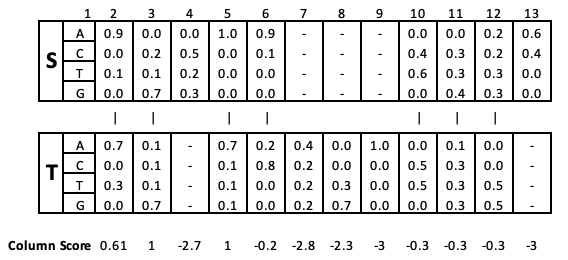
\includegraphics{HW3_Align}
\caption{Alignment of two profiles}
\end{centering}
\end{figure}

\begin{figure}[h!]
\begin{centering}
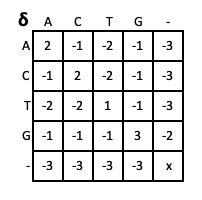
\includegraphics{HW3_Delta}
\caption{Scoring scheme}
\end{centering}
\end{figure}


\end{enumerate}
\end{document} 